\documentclass[crop,tikz]{standalone}
\makeatletter
\usetikzlibrary{3d}
\begin{document}


% kepler_2_particles
  \begin{tikzpicture}[scale=4]
    \coordinate (O) at (0,0,0);
    \draw[thick] (-1.1,0,0) -- (O);
    \draw[thick] (0,-0.75,0) -- (O);
    \draw[thick] (0,0,-1) -- (O);
    \draw[->, >=latex, thick] (O) -- (1.1,0,0) node[right]{$y$};
    \draw[->, >=latex, thick] (O) -- (0,1,0) node[left]{$z$};
    \draw[->, >=latex, thick] (O) -- (0,0,1) node[left]{$x$};
    
    % Define coordinates of the two bodies
    \pgfmathsetmacro{\px}{-1};
    \pgfmathsetmacro{\py}{0.5};
    \pgfmathsetmacro{\pz}{0.5};
    \pgfmathsetmacro{\dx}{1};
    \pgfmathsetmacro{\dy}{0.3};
    \pgfmathsetmacro{\dz}{-1};
    \coordinate (M1) at (\px,\py,\pz);
    \coordinate (M2) at (\dx,\dy,\dz);
    
    % Draw the bodies
    \fill[fill=blue!50!black!50] (M1) circle (1pt);
    \fill[fill=red!50!black!50] (M2) circle (1pt);
    
    % Draw the positions of each body relative to the origin
    \draw[->,>=stealth] (O) -- (M1) node[pos=0.7, above, yshift=1mm]{$\mathbf{r}_1$};
    \draw[->,>=stealth] (O) -- (M2) node[pos=0.7, above, yshift=1mm]{$\mathbf{r}_2$};
    
    % Draw the projections of both bodies onto the plane
    \draw[dashed] (M1) -- (\px, 0, \pz);
    \draw[dashed] (\px, 0, \pz) -- (\px, 0, 0);
    %\draw[dashed] (\px, 0, \pz) -- (0, 0, \pz);
    \draw[dashed] (M2) -- (\dx, 0, \dz);
    \draw[dashed] (\dx, 0, \dz) -- (\dx, 0, 0);
    %\draw[dashed] (\dx, 0, \dz) -- (0, 0, \dz);
    
    
    %% Draw the vector from body 1 to body 2
    %\draw[->,>=stealth] (M1) -- (M2) node[pos=0.6, above]{$\vec{r}$};
    
    % Provide the masses
    \node at (M1) [left, xshift=-0.75mm]{$m_1$};
    \node at (M2) [right, xshift=1mm]{$m_2$};
  \end{tikzpicture}

\newpage
% reduced_mass_system
  \begin{tikzpicture}[scale=4]
	% Draw a sample trajectory that the particle takes
	\begin{scope}
		% Draw "rings" where the trajectory "passes through the horizontal plane"
		\foreach \t in {50, 150} {
			\pgfmathsetmacro{\x}{-0.35*cos(\t)+\t/180}
			\pgfmathsetmacro{\y}{cos(\t)^2-0.1*sin(\t)}
			\pgfmathsetmacro{\z}{2-cos(\t)^2}
			\begin{scope}[canvas is xz plane at y=\y]
				\draw[red!80!black!80] (\x,\z) circle (0.2 mm);
 			\end{scope}
 		}
 		
		% Define times at which the trajectory looks like it passes through
		% the planes
		\pgfmathsetmacro{\tlim}{105}
		\pgfmathsetmacro{\tlimTwo}{198}
		\pgfmathsetmacro{\tfinal}{255}
		
		% Flow from the reduced particle through the horizontal plane
		% up until passing through the vertical plane facing the screen
  		\begin{scope}[black, dashed, ->, >=stealth]
  			\pgfplothandlerlineto
  			\pgfplotfunction{\t}{0,1,...,\tlim}
       		{\pgfpointxyz {-0.35*cos(\t)+\t/180}{cos(\t)^2-0.1*sin(\t)}{2-cos(\t)^2}} 
       		\pgfusepath{stroke}
		\end{scope}
  		
  		% Flow in the background until coming back up front
  		\pgfmathsetmacro{\tlimPlusOne}{\tlim+1}
  		\pgfmathsetmacro{\tlimPlusTwo}{\tlim+2}
		\begin{scope}[black!40, dashed, ->, >=stealth]
  			\pgfplothandlerlineto
			\pgfplotfunction{\t}{\tlimPlusOne,\tlimPlusTwo,...,\tlimTwo}
       		{\pgfpointxyz {-0.35*cos(\t)+\t/180}{cos(\t)^2-0.1*sin(\t)}{2-cos(\t)^2}} 
       		\pgfusepath{stroke}
		\end{scope}
		
		% Finish the flow
    		\pgfmathsetmacro{\tlimTwoPlusOne}{\tlimTwo+1}
  		\pgfmathsetmacro{\tlimTwoPlusTwo}{\tlimTwo+2}
		\begin{scope}[black, dashed, ->, >=stealth]
  			\pgfplothandlerlineto
			\pgfplotfunction{\t}{\tlimTwoPlusOne,\tlimTwoPlusTwo,...,\tfinal}
       		{\pgfpointxyz {-0.35*cos(\t)+\t/180}{cos(\t)^2-0.1*sin(\t)}{2-cos(\t)^2}} 
       		\pgfusepath{stroke}
		\end{scope}
    \end{scope}
  
  	
    \coordinate (O) at (0,0,0);
    \draw[thick] (-1.1,0,0) -- (O);
    \draw[thick] (0,-0.75,0) -- (O);
    \draw[thick] (0,0,-1) -- (O);
    \draw[->, >=latex, thick] (O) -- (1.1,0,0) node[right]{$y$};
    \draw[->, >=latex, thick] (O) -- (0,1,0) node[left]{$z$};
    \draw[->, >=latex, thick] (O) -- (0,0,1) node[left]{$x$};
  	
	% Define the position of the reduced mass particle
  	\coordinate (M) at (-0.35,1,1);
	
	% Draw the bodies
    \fill[fill=black!50] (O) circle (1pt);
    \fill[fill=green!50!black!50] (M) circle (0.5pt);
    
    % Draw the position of the reduced mass body relative to the other body
    \draw[->,>=stealth] (O) -- (M) node[pos=0.7, above, yshift=+1mm]{$\mathbf{r}$};
	%\draw[dashed] (M) -- (-0.35, 0, 1);
    %\draw[dashed] (-0.35, 0, 1) -- (-0.35, 0, 0);
    %\draw[dashed] (-0.35, 0, 1) -- (0, 0, 1);    
    
    % Draw the anchor at the origin (mass m1 + m2) and the reduced mass particle
  	\node at (O) [anchor=north west, xshift=1mm]{$m_1 + m_2$};
    \node at (M) [left]{$\mu^*$};
  \end{tikzpicture}

\newpage
% kepler_solution
  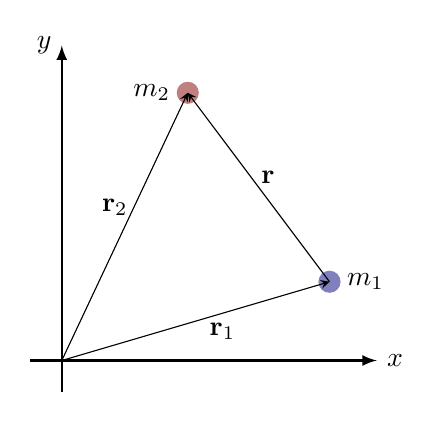
\begin{tikzpicture}[scale=4]
    \coordinate (O) at (0,0);
    \draw[thick] (-0.1,0) -- (O);
    \draw[thick] (0,-0.1) -- (O);
    \draw[->, >=latex, thick] (O) -- (1,0) node[right]{$x$};
    \draw[->, >=latex, thick] (O) -- (0,1) node[left]{$y$};
    
    % Define coordinates of the two bodies
    \pgfmathsetmacro{\px}{0.85};
    \pgfmathsetmacro{\py}{0.25};
    \pgfmathsetmacro{\dx}{0.4};
    \pgfmathsetmacro{\dy}{0.85};
    \coordinate (M1) at (\px,\py);
    \coordinate (M2) at (\dx,\dy);
    
    % Draw the bodies
    \fill[fill=blue!50!black!50] (M1) circle (1pt);
    \fill[fill=red!50!black!50] (M2) circle (1pt);
    
    % Draw the positions of each body relative to the origin
    \draw[->,>=stealth] (O) -- (M1) node[pos=0.6, below, yshift=0mm]{$\mathbf{r}_1$};
    \draw[->,>=stealth] (O) -- (M2) node[pos=0.6, left, yshift=-1mm]{$\mathbf{r}_2$};
    
    % Draw the vector from body 1 to body 2
    \draw[->,>=stealth] (M1) -- (M2) node[pos=0.55, right]{$\mathbf{r}$};
    
    % Provide the masses
    \node at (M1) [right, xshift=1mm]{$m_1$};
    \node at (M2) [left, xshift=-1mm]{$m_2$};
  \end{tikzpicture}

\end{document}